%---Linda

The post processing is based on the correction of the raw data.
Firstly, we have to process the data with the corresponding data of the base station data to get a higher accurancy of the GPS data.
The nearest base station is Statens Kartverks SatRef located on Platåberget with a distance between 14 km and 20 km depending on the mass balance stake.
In the following the mass balance stake is only named stake and the pole with the rover will be shortend to the name rover.
\medskip

% 2 different methods:
In the previous reports the post processing was done with the commercial software \textit{Trimble Business Center} (TBC). 
In our report we use a new method for the postprocessing. 
This method is an open source alternative which is available for different system softwares. 
The TBC is only available on a windows system and needs a licens. 
We operate both methods to compare the results of both methods.
The differences for every stake are given in the table \ref{GPS:tab:diff_tab}.
The direction for Northing and Easting varies randomly in the direction.
Because of this, it is not possible to determine a bias for each component.
This results in a mean difference of the absolut values with 0.15 m in the Northing, 0.14 m in the Easting and 0.24 m in the Elevation.
\medskip

% steps of the post processing:
While the post processing with the usual method in the TBC all steps from section 5 in Gölles (2012) are done.
For each day the data file from the measurements and the corresponding base station data file is imported. 
We have data for the days of year (doy) 070, 072, 074 and 075.
All files from the base station are in the .o18-format. 
The data from the reciever have the .t02 format. 
After the post processing the results from the are stored in a .csv-file.
\medskip

The open source post processing requires different processing steps.
First of all the raw data file has to be transformed from the original Trimble format .t02 to the .tdg-format, because .t02-files are not readable for the final post processing program.
This transformation was done with the programm  runpkr00  which is available on the website of unavco \url{http://kb.unavco.org/kb/article/trimble-runpkr00-v5-40-latest-version-mac-osx-10-7-windows-xp-7-linux-solaris-744.html}.
The used command is 
\begin{verbatim} 
runpkr00 -g -d filename.t02 
\end{verbatim}.
Due to problems with the package we had to do a manual transformation of the package.
To provide the correct file format for the last post processing step we use the toolkit teqc.
This toolkit is also available on the website of unavco \url{https://www.unavco.org/software/data-processing/teqc/teqc.html}.
Then the file can be converted by another commad using
\begin{verbatim}
./teqc +nav filename.nav +obs filename.obs filename.tgd
\end{verbatim} 
to an observation (.obs) and navigation (.nav) file.
After that it is necessary to download also the base station data from the platform \url{http://ftp.statkart.no/}.
The final step in the post processing of the GPS data is done with the open source program package \textit{RTKLIB}.
This package is available for the download in the website \url{http://www.rtklib.com/rtklib.htm}.
In this package we use the executable rtkpost.exe in the subdirectory \textit{/bin} of the downloaded full package with source Programs with the version 2.4.2.
In this software the two navigation file from the receiver and the base station as well as the observation file from the receiver has to be read in.
For this method the .n18-format from the basestation is needed as comparable navigation file.
The next steps are consistent to the description on the website \url{https://docs.emlid.com/reach/common/tutorials/gps-post-processing/}.
For this we had to modify the settings of rtkpost.exe and load the three required files. 
The final output after the post processing is a position file (.pos). 
This file includes for every time step the post processed position in longitude and latitude.
Then we calculate a median over all time steps to get an average position for every measurement.
Because we consistenly use the UTM coordinate system, we transform the lon/lat coordinates by using the python function \textit{from\_latlon}.
All the analysis in this report is made with python.
\medskip

% theory of trimble post processing/
%...GNSS processing theory:
There are five different GNSS constellations GPS, GLONASS, QZSS, COMPASS and Galileo.
The Real-time Kinematic (RTK) of Trimble.
The orbit of the satellites is approximately in 20000 km.
When the position of the satellite is known, the position of the receiver is calculated by trilateration based on the measured distance between receiver and each satellite.
The position of the satellite is broadcast as a ephemerides, which is a specific positioning.
For reducong the errors by different sources the receiver need a additional source with precise positions, clock offsets and goog correction of atmosphic disturbances. 
Differential positioning is used to reduce the errors by orbit and atmosphere, which ar e similar for both receiver. 
The Carrier phase is used for the measurements because it has a smaller wavenegth than the Pseudorandom Noise (PRN) code signal.

%The carrier phase measurement is the difference in the phase of the received signal and the phase of an equivalent signal generated from the receiver’s oscillator or clock.

%Traditional GNSS processing engines used the combination of reference and rover data to attempt to “fix” the number of whole wavelengths between the rover and satellites.

This process is done in two steps by generating a 'float' solution an and resolve an integer value. 
Wheh it is sucessful the solution is defined as 'fixed'.
The transition from 'float' to 'fixed' is the initialization.

%The float solution was often maintained for a considerable amount of time when working in a difficult environment or with a long baseline, and was followed by an instantaneous switch to a fixed solution. Hence, the convergence from float to fixed was highly polarized. There were a number of disadvantages to the float/fixed approach for integer ambiguity resolution. For one thing, the user was unable to extract usable positions until the receiver had converged on a fixed solution. Also, there was the possibility of an incorrect solution where the processing engine selected the wrong set of integer ambiguities. In this event, the correct integer set was discarded and could not be selected until the search was repeated. For RTK, this resulted in a position outlier being reported with unrealistically good precisions for many seconds until detected by an automated integrity check.

A slow convergence of the solution is possible for longer baselines or shielding of the signal by objects in the surrounding.

By mistake it is possible that during the post processing process a wrong fixed values is hold which can lead to an unnormal high position error.

%---post processingn application
The TBC use automatically the best way to process the position data. 
It is distingushed in short and long baselines.
Baselines are determined by the distance between rover and reference station.
For longer baselines the errors have to be reduced with an additional approach like a model.
For different settings and situations the TBC used different approaches for the tropospheric and ionospheric errors and choose the right combinaion of different applications.

\citep{Trprocess}.

% therory of the open source post processing
The header with the settings for the post processing is available in the appendix.

\begin{figure}[H]
    \centering
    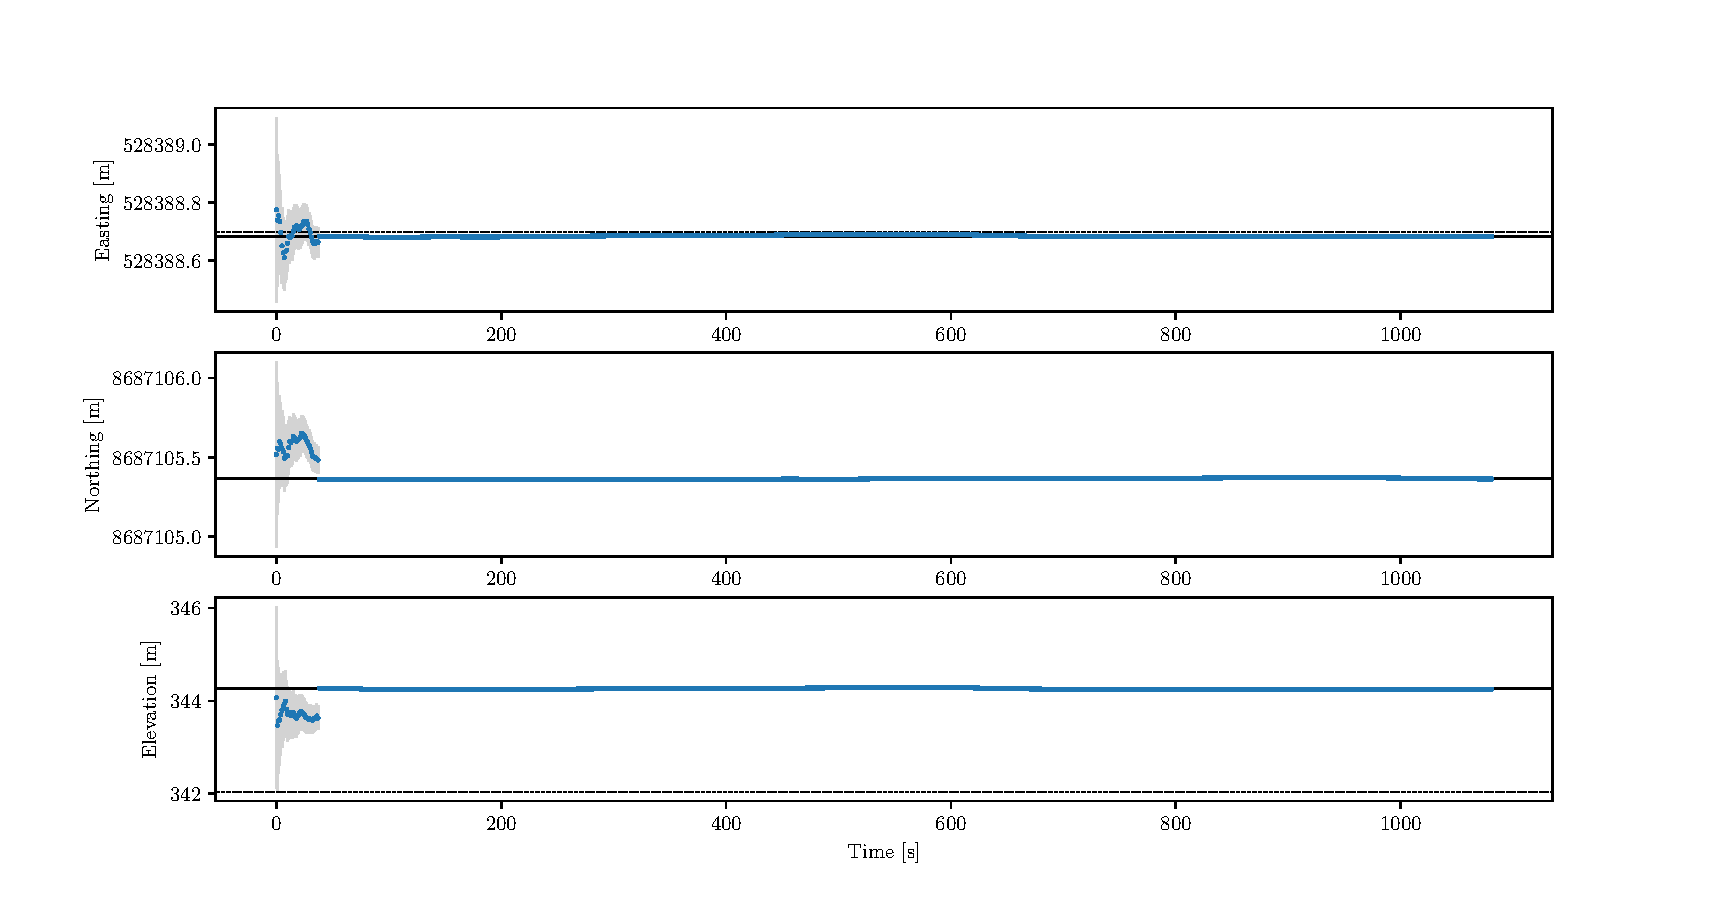
\includegraphics[width=\textwidth]{./figs/timeseries/46250700_corr-T1-i-2017_Timeseries-east-north-elev.pdf}
    \caption{First of two measurements of position of stake T1. Compare to Fig.~\ref{GF:fig:T1-ii_timeseries}.}
    \label{GF:fig:T1-i_timeseries}
\end{figure}


\begin{figure}[H]
    \centering
    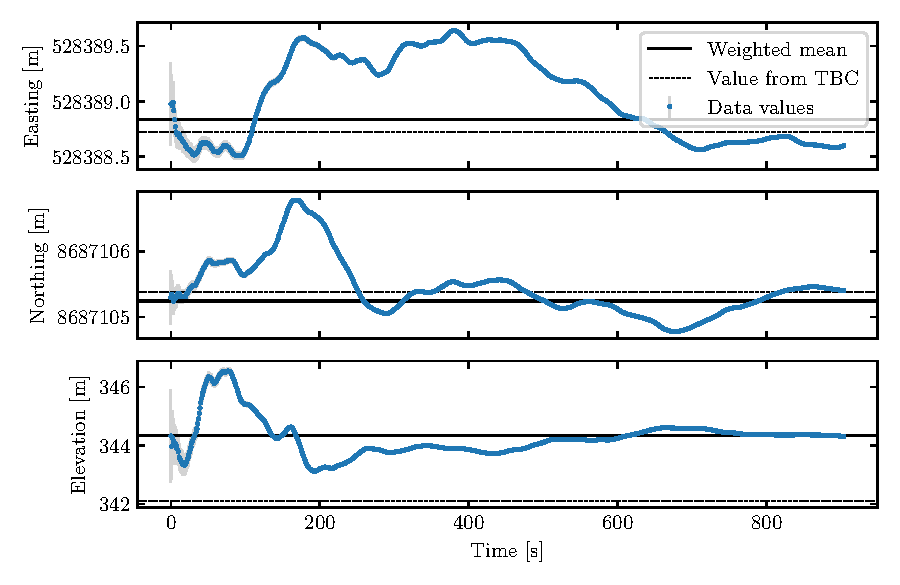
\includegraphics[width=\textwidth]{./figs/timeseries/46250723_corr-T1-ii-2017_Timeseries-east-north-elev.pdf}
    \caption{Second of two measurements of position of stake T1. Compare to Fig.~\ref{GF:fig:T1-i_timeseries}.}
    \label{GF:fig:T1-ii_timeseries}
\end{figure}

Then it was calculated the weighted average to get one position value for every stake.

% error correction of the post processed data:
The post processed data with the base station data are not the final data. 
To get the final, we have to make the stake correction include the different aspects from our measurement setup (see section setup).
We subtract the distance between the rover and the stake from the northing component.
Also it was necessary to correct the position on the ice surface with the inclination of the stake. 
For this, we consider the inclination of the stake and calculate the error dependent on the height of the stake and the direction of the inclination.
The raw data from our measurements which are relevant for our stake corrections are in the appendix in table \ref{GPS:tab:fb_others_tab}.
\medskip

The calculations for the error propagation follow the common rule.

\begin{figure}
\centering
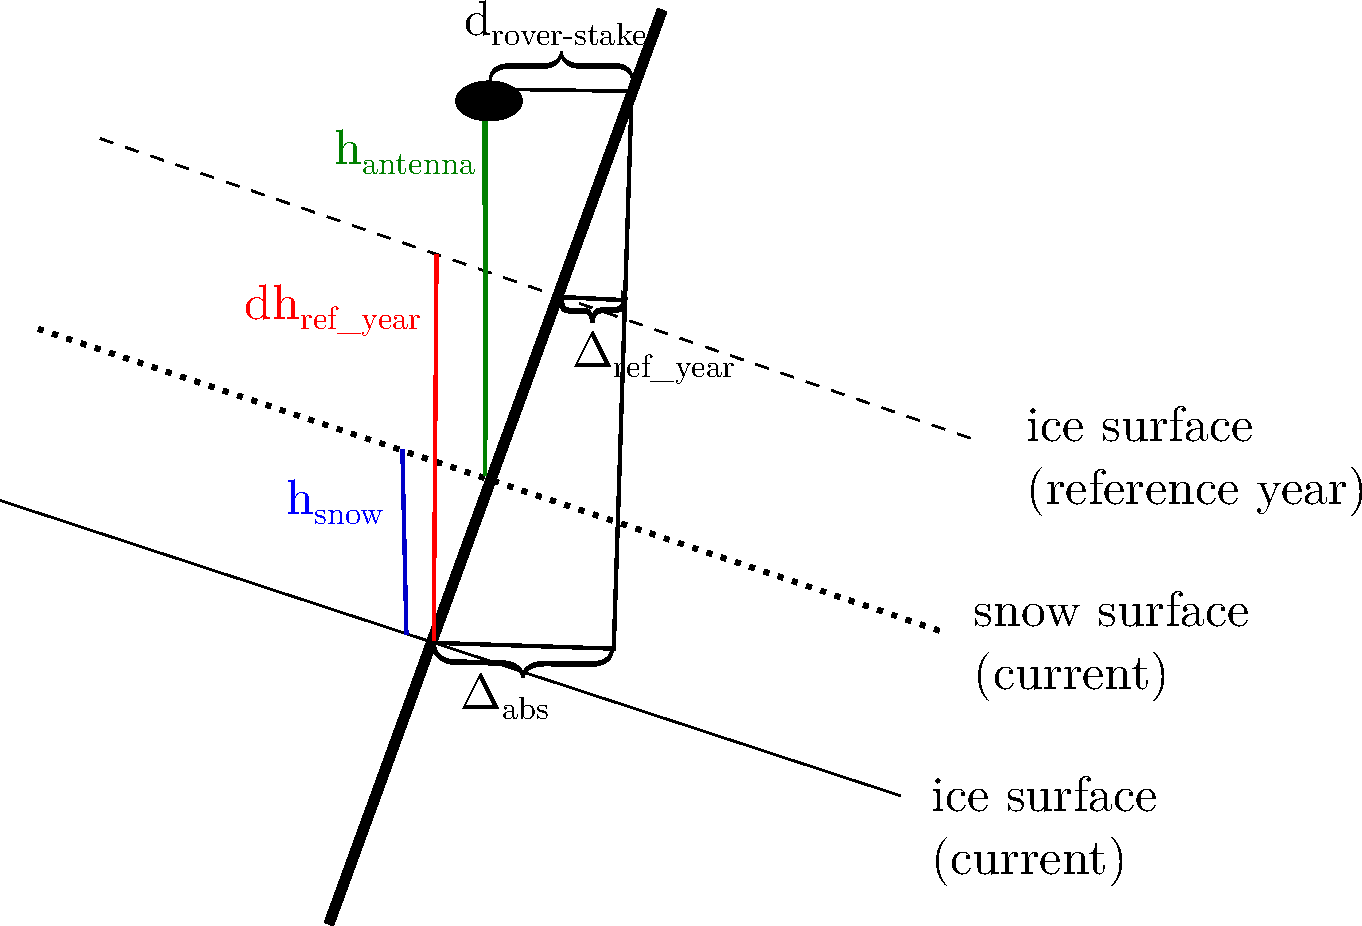
\includegraphics[width=0.9\linewidth]{./figs/pictures/schematic_setup.pdf}
\caption{Schematic figure of the relevant parameter in the measurment setup.}
\end{figure}

% name accurancies of the final data:
The accurancy of the post processed postions with the base station data is decreasing with a increasing distance to the base station. 
But this error is at least one order of magnitude smaller than the other errors. 
The other accurancies are determined by the quality of our measurements \ref{GPS:tab:errors}.

\begin{table}[h]
	\caption{Used error values for the error propagation.}
	\centering
	\begin{tabular}{lc}
	\toprule
        error &  value \\
	\midrule
    $ \delta_{\alpha} $ &  3$^{\circ}$ \\
    $ \delta_{\phi} $ &  22.5$^{\circ}$ \\
    $ \delta_{h_{snow}}$ &  0.02 m \\
    $ \delta_{h_{antenna}} $ &  0.05 m \\
    $ \delta_{dh_{year,2018}} $ &  0.10 m \\
    $ \delta_{d_{rover-stake}} $ &  0.02 m \\
    $ \overline{\delta_{\Delta_{north}}} $ & 0.40 m \\
    $ \overline{\delta_{\Delta_{east}}} $ & 0.19 m \\
    $ \overline{\delta_{\Delta_{elev}}} $ & 0.89 m \\
    \bottomrule
\end{tabular}
	\label{GPS:tab:errors}
\end{table} 


% formulars stake correction
\begin{equation}
	\Delta_{\text{abs}} = (h_{\text{snow}} + h_{\text{antenna}}) * sin(\alpha)
\end{equation}

\begin{equation}
	\Delta_{\text{north}} = - (\Delta_{\text{abs}} * cos(\phi)) - d_{\text{rover-stake}}
\end{equation}

\begin{equation}
	\Delta_{\text{east}} = - \Delta_{\text{abs}} * sin(\phi)
\end{equation}

\begin{equation}
	\Delta_{\text{elev,os}} = - (h_{\text{snow}} + h_{\text{antenna}}) 
\end{equation}

\begin{equation}
	\Delta_{\text{elev,TBC}} = - h_{\text{snow}} 
\end{equation}

% formulars error propagation

\begin{equation}
	\delta_{\Delta_{\text{abs}}} = \sqrt{(h_{\text{snow}} + h_{\text{antenna}})^2 * \delta_{\alpha}^2 * cos^2(\alpha) + (\delta_{h_{\text{snow}}}^2 + \delta_{h_{\text{antenna}}}^2) * \sin^2(\alpha)}
\end{equation}

\begin{equation}
	\delta_{\Delta_{\text{north}}} = \sqrt{\delta_{\Delta_{\text{abs}}}^2 * cos^2(\phi) + \Delta_{\text{abs}}^2 * \delta_{\phi}^2 * sin^2(\phi) + \delta_{d_{\text{rover-stake}}}^2}
\end{equation}

\begin{equation}
	\delta_{\Delta_{\text{east}}} = \sqrt{\delta_{\Delta_{\text{abs}}}^2 * sin^2(\phi) + \Delta_{\text{abs}}^2 * \delta_{\phi}^2 * cos^2(\phi)}
\end{equation}

\begin{equation}
	\delta_{\Delta_{\text{total,north}}} = \sqrt{\delta_{\Delta_{\text{ts,north}}}^2 + \delta_{\Delta_{\text{north}}}^2}
\end{equation}

\begin{equation}
	\delta_{\Delta_{\text{total,east}}} = \sqrt{\delta_{\Delta_{\text{ts,east}}}^2 + \delta_{\Delta_{\text{east}}}^2}
\end{equation}

\begin{equation}
	\delta_{\Delta_{\text{total,elev}}} = \sqrt{\delta_{\Delta_{\text{ts,elev}}}^2 +\delta_{\Delta_{\text{elev}}}^2}
\end{equation}

% for the referenced position
To calculate the actual velocity it is necessary to reference the location of the stake to the ice surface elevation of the referenced year. 
This has been done for the years 2015, 2016 and 2017.
 
\begin{equation}
\delta_{\Delta_{year,2018}} = \sqrt{\left|(h_{\text{snow}} + h_{\text{antenna}} - dh_{year,2018})^2\right| * \delta_{\alpha}^2 * cos^2(\alpha)\\
+ (\delta_{h_{\text{snow}}}^2 + \delta_{h_{\text{antenna}}}^2 + \delta_{dh_{year,2018}}^2) * \sin^2(\alpha)}
\end{equation}

\begin{equation}
	\delta_{\Delta_{year, \text{elev}}} = \sqrt{\delta_{h_{\text{snow}}}^2 + \delta_{h_{\text{snow}}}^2 + \delta_{h_{\text{snow}}}^2}
\end{equation}

\begin{equation}
	\Delta_{year,2018} = (h_{\text{snow}} + h_{\text{antenna}} - dh_{year,2018}) * sin(\alpha)
\end{equation}

The final data show the actual position of the stakes on this years ice surface.

\begin{table}[H]
	\caption{Final positions after the open source post processing and stake correction with the error.}
	\centering
	\begin{tabular}{lrrrrrr}
\toprule
        Name &  Northing [m] &  Error Northing [m] &  Easting [m] &  Error Easting [m] &  Elevation [m] &  Error Elevation [m] \\
\midrule
    BL2-2016 &    8686150.74 &                0.16 &    523049.41 &               0.11 &         436.89 &                 0.48 \\
    BL2-2018 &    8686149.82 &                0.01 &    523051.47 &               0.03 &         437.74 &                 0.06 \\
    BL3-2016 &    8686091.51 &                0.27 &    523544.75 &               0.13 &         490.82 &                 0.25 \\
    BL3-2018 &    8686091.17 &                0.42 &    523545.34 &               0.10 &         491.39 &                 1.03 \\
    BL4-2018 &    8686098.58 &                0.17 &    524179.27 &               0.15 &         573.74 &                 0.20 \\
  BL4-i-2016 &    8686098.47 &                0.26 &    524179.80 &               0.19 &         571.65 &                 0.20 \\
 BL4-ii-2016 &    8686098.39 &                1.30 &    524179.92 &               0.31 &         571.36 &                 4.82 \\
  BL5-i-2017 &    8686130.74 &                0.09 &    524644.27 &               0.01 &         628.63 &                 0.09 \\
 BL5-ii-2017 &    8686130.74 &                0.28 &    524644.28 &               0.15 &         628.56 &                 0.75 \\
     T1-2018 &    8687106.55 &                0.32 &    528388.42 &               0.07 &         341.59 &                 0.24 \\
   T1-i-2017 &    8687105.69 &                0.13 &    528388.68 &               0.18 &         341.26 &                 0.12 \\
  T1-ii-2017 &    8687105.58 &                0.45 &    528388.84 &               0.44 &         341.38 &                 0.65 \\
     T2-2016 &    8687321.31 &                0.42 &    527951.88 &               0.14 &         394.88 &                 2.34 \\
     T2-2018 &    8687319.62 &                0.28 &    527951.35 &               0.27 &         395.86 &                 1.61 \\
   T2-i-2017 &    8687321.37 &                0.30 &    527950.58 &               0.25 &         395.22 &                 0.34 \\
  T2-ii-2017 &    8687320.98 &                1.31 &    527951.01 &               0.26 &         394.74 &                 1.26 \\
     T3-2017 &    8687273.11 &                0.11 &    527598.29 &               0.01 &         422.59 &                 0.07 \\
     T4-2016 &    8687138.56 &                0.47 &    527123.97 &               0.34 &         486.80 &                 1.07 \\
     T4-2018 &    8687137.72 &                1.05 &    527124.90 &               0.37 &         487.94 &                 2.33 \\
     T5-2016 &    8686938.28 &                0.57 &    526692.25 &               0.25 &         534.57 &                 0.72 \\
     T5-2018 &    8686937.68 &                0.21 &    526690.76 &               0.21 &         535.09 &                 0.45 \\
     T6-2016 &    8686675.01 &                0.51 &    526250.17 &               0.22 &         561.87 &                 0.89 \\
     T6-2018 &    8686674.78 &                0.48 &    526246.88 &               0.39 &         560.47 &                 0.79 \\
     T7-2015 &    8686578.89 &                0.24 &    525858.01 &               0.17 &         615.10 &                 0.71 \\
     T7-2017 &    8686579.37 &                0.19 &    525858.38 &               0.04 &         615.95 &                 0.71 \\
     T8-2017 &    8686471.52 &                0.48 &    525523.82 &               0.13 &         649.73 &                 1.02 \\
\bottomrule
\end{tabular}

	\label{GPS:tab:os_tab}
\end{table}

For the difference between the two different methods is not systematic and in the avereage of the absolute values in the order of centimeters with 0.09 m for the northing, 0.05 m for thehe  easting and 0.24 m for the elevation. This is mainly caused by a few unclear values after the post processing. The meadian of the northing and eastind difference is about 0.01 m and for the elevation only 0.07 m. For the comparison the TBC post processed coordinates are in the appendix in table \ref{GPS:tab:tbc_tab}.
The differences for northing, easting and elevation for every stake is displayed in a table in the appendix in table \ref{GPS:tab:diff_tab}. 
